{\textbf{中断}}概念的出现是计算机系统结构设计中的一个重大变革。

第7章会讲到程序中断方式,某一外部设备的数据准备就绪后,它``主动''向CPU发出请求中断的信号,请求CPU暂时中断目前正在执行的程序而进行数据交换。

\textbf{当CPU响应这个中断时,}便暂停运行主程序,并自动转移到该设备的中断服务程序。

\textbf{当中断服务程序结束以后,}CPU又回到原来的主程序。其实,计算机在运行过程中,除了会遇到I/O中断外,还有许多意外事件发生,如突然断电,机器硬件突然出现故障等。中断处理过程的详细流程,如下图所示。

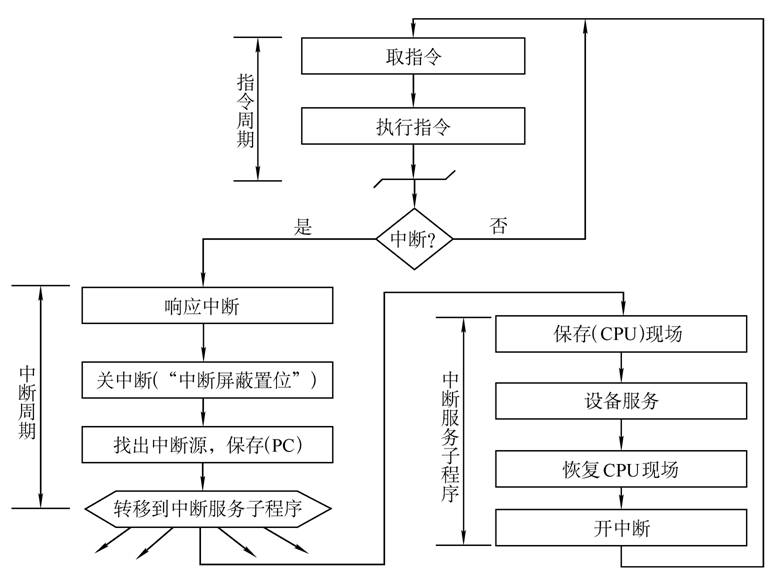
\includegraphics[width=3.43750in,height=2.55208in]{png-jpeg-pics/7C2E026DFCC048F8EF1C3A969D5AE3F2.png}

\textbf{图解:}当CPU执行完一条现行指令时,如果外部设备向CPU发出中断请求,那么CPU在满足响应条件的情况下,将发出中断响应信号,与此同时关闭中断(``中断屏蔽''触发器置``1''),表示CPU不再受理另外一个设备的中断。这时,\textbf{CPU将寻找中断请求源是哪一个设备,并保存CPU自己的程序计数器(PC)的内容。}然后,它将\textbf{转移到处理该中断源的中断服务程序}。CPU在保存现场信息、设备服务(如交换数据)以后,将\textbf{恢复现场信息}。这些动作完成以后,\textbf{开放中断}(``中断屏蔽''触发器置``0''),并\textbf{返回到原来被中断的主程序的下一条指令}。

{关于中断系统的讲解,详见书籍《计算机组成原理高分笔记》。}
